\documentclass[12pt]{article}

\usepackage{fullpage}
\usepackage{graphicx, rotating, booktabs} 
\usepackage{times} 
\usepackage{natbib} 
\usepackage{indentfirst} 
\usepackage{setspace}
\usepackage{grffile} 
\usepackage{hyperref}
\usepackage{adjustbox}
\usepackage{amsmath}
\usepackage{siunitx}
\usepackage{multirow}
\setcitestyle{aysep{}}


\singlespace
\title{\textbf{Appendix: Public Attitudes Towards Military Alliances}}
\author{}
\date{\today}

\bibliographystyle{apsr}

\begin{document}

\maketitle 

\doublespace 


\section{Marginal Mean Alliance Support by Foreign Policy Disposition} 


The manuscript reports analyses with partisan subgroups, as well as foreign policy dispositions within each party. 
In this section of the appendix, I report subgroup analyses by foreign policy disposition across partisanship. 
\autoref{fig:hawk-plots} and \autoref{fig:isolation-plots} show the distribution of alliance attitudes for hawkishness and isolationism. 


First, hawkish individuals are more likely to support alliance formation and maintenance, regardless of specific alliance characteristics. 
Hawks are also more responsive to cues from Republican Senators and the Joint Chiefs of Staff. 
Doves pay more attention to cues from Democratic Senators.
The results in the manuscript clearly show the sources of these partisan differences, as Republicans are usually more hawkish. 


\begin{figure}
	\centering
		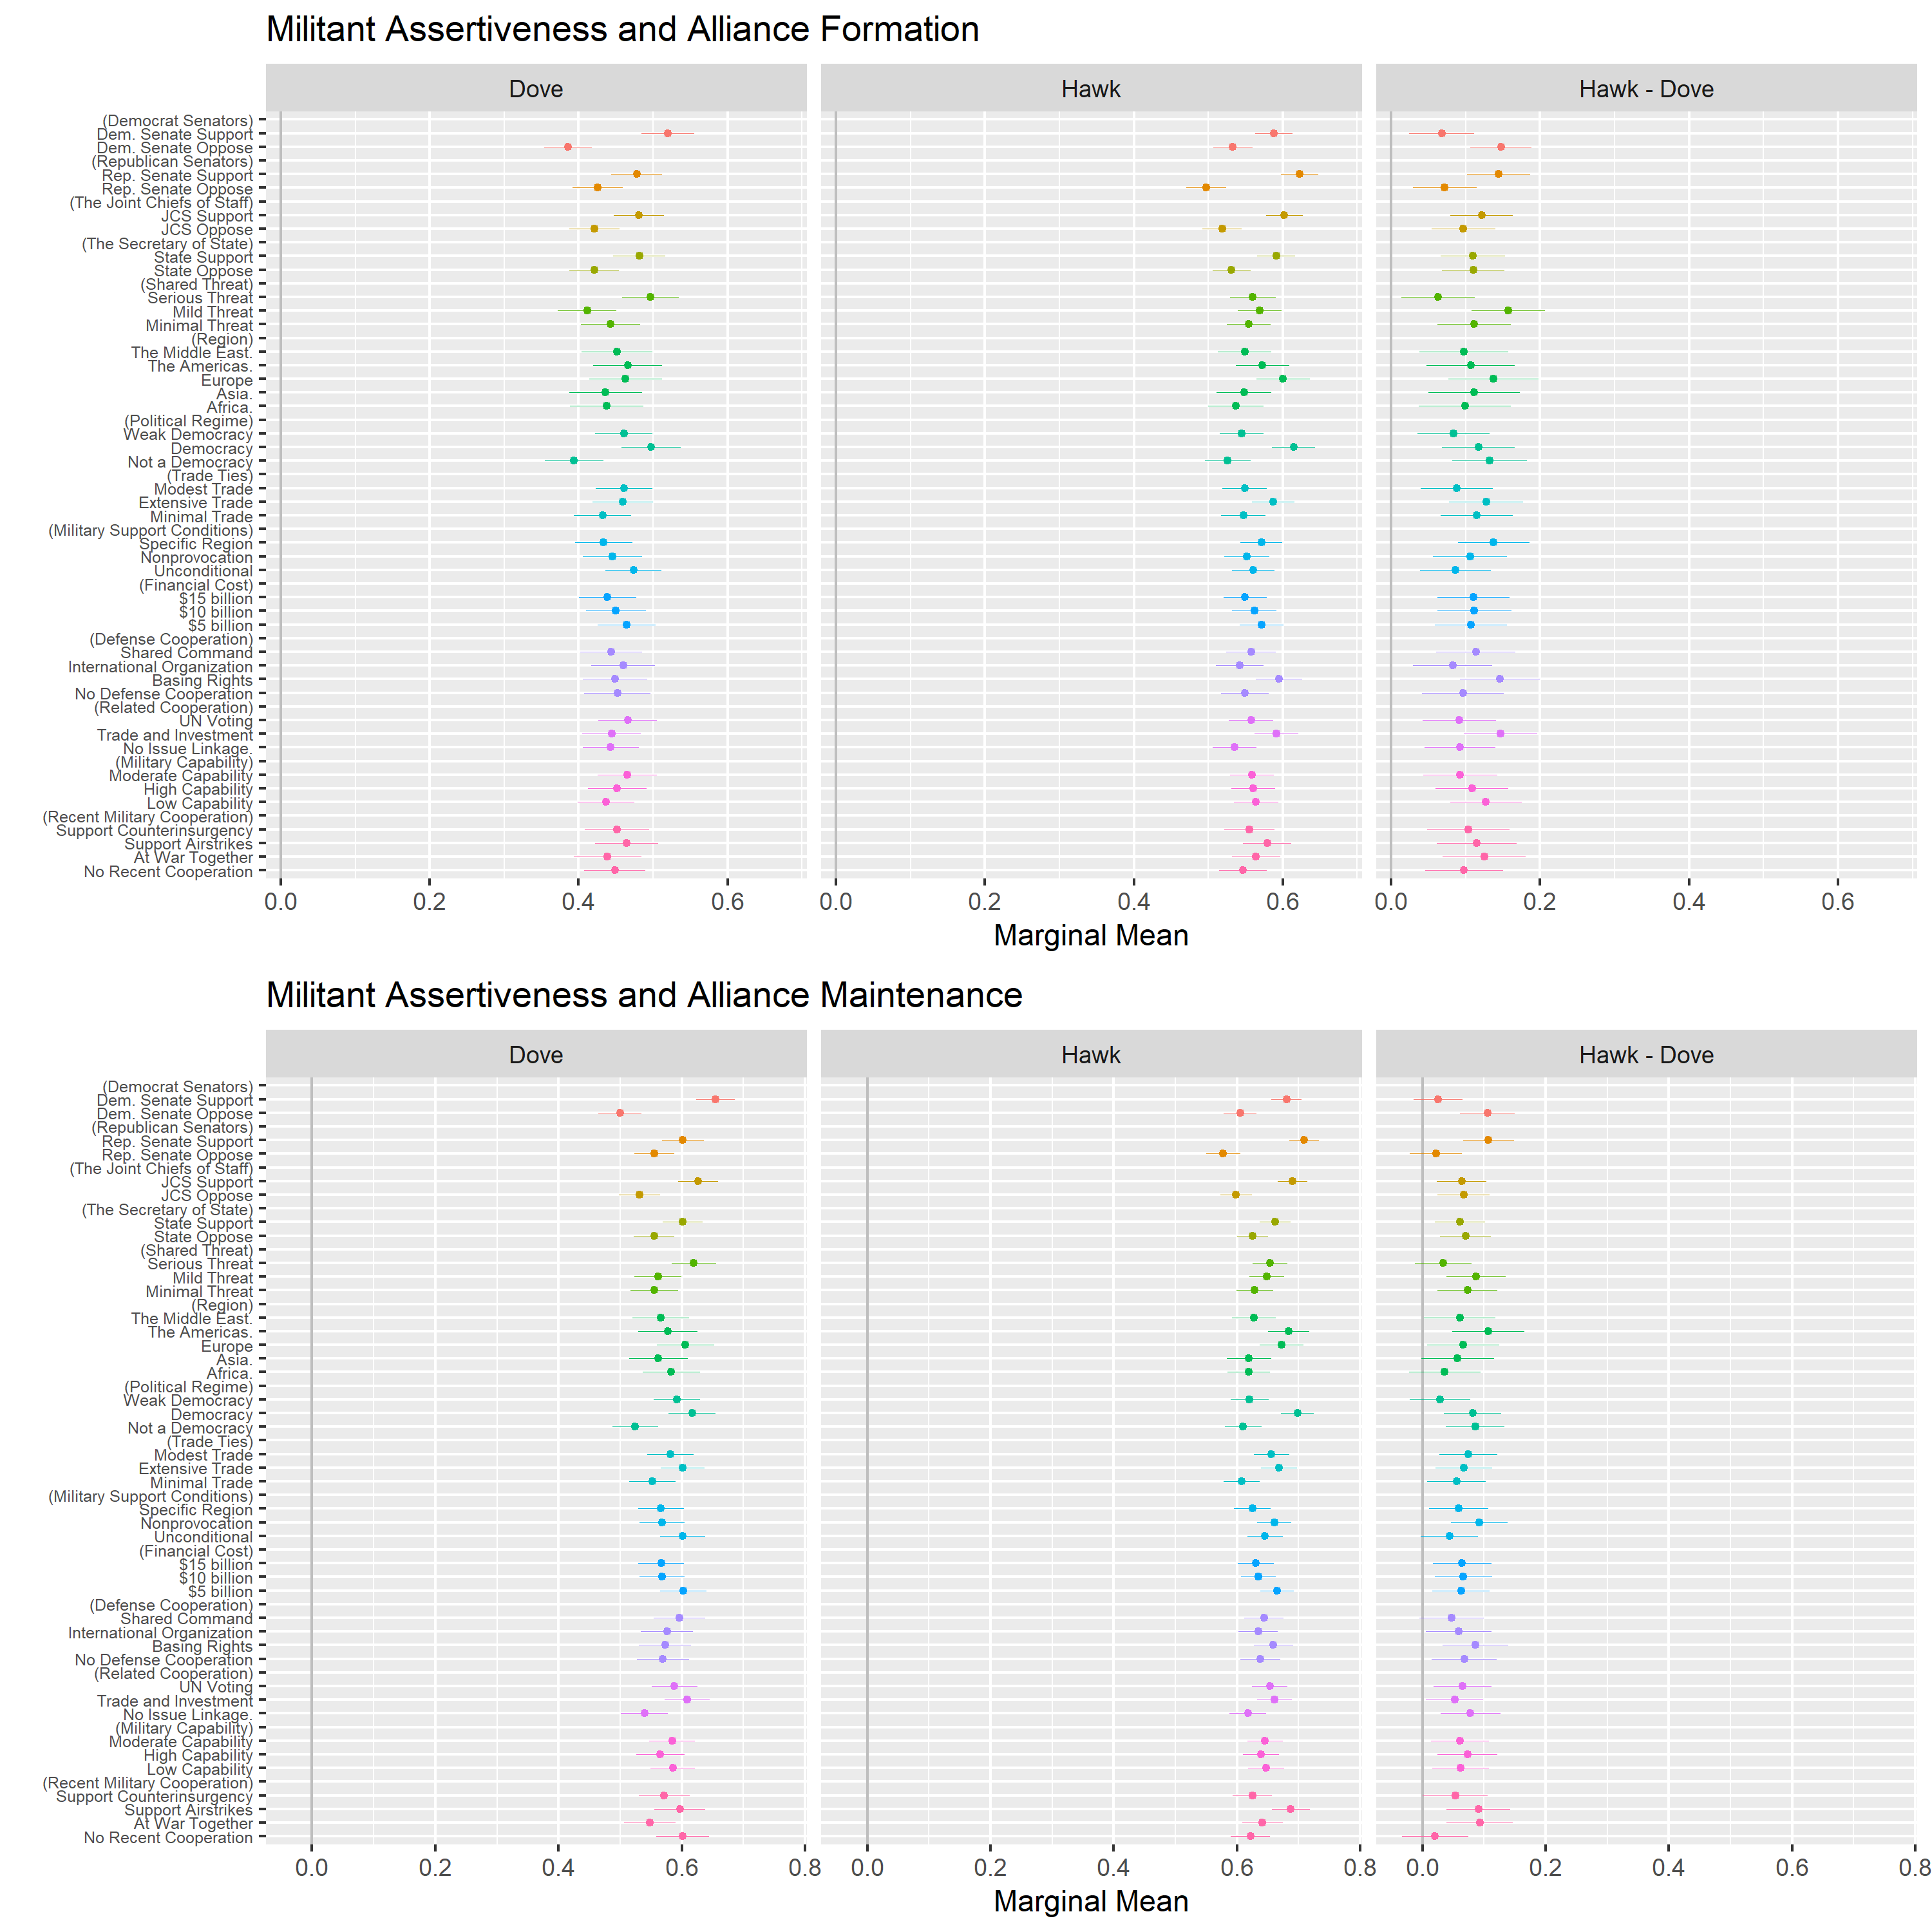
\includegraphics[width=0.95\textwidth]{hawk-plots.png}
	\caption{Marginal means of support for forming or maintaining a hypothetical alliances by militant internationalism. For each experiment, the left two panels plot the marginal mean of support for alliance participation among hawks and doves under different alliance treatments. The rightmost panel plots the difference between these groups. Components marked with abbreviated labels to make the plot more legible.}
	\label{fig:hawk-plots}
\end{figure}


Isolationism does not reduce baseline support for alliances, but it does change individual responses to elite cues. 
Internationalist respondents are more receptive to elite cues, as \autoref{fig:isolation-plots} shows. 
Although isolationists and internationalists have similar levels of support for alliance participation across most alliance attribute, marginal mean support among internationalists diverges strongly in response to elite support or opposition. 
As a result, isolationists have higher alliance support than internationalists when elites oppose treaty formation. 


\begin{figure}
	\centering
		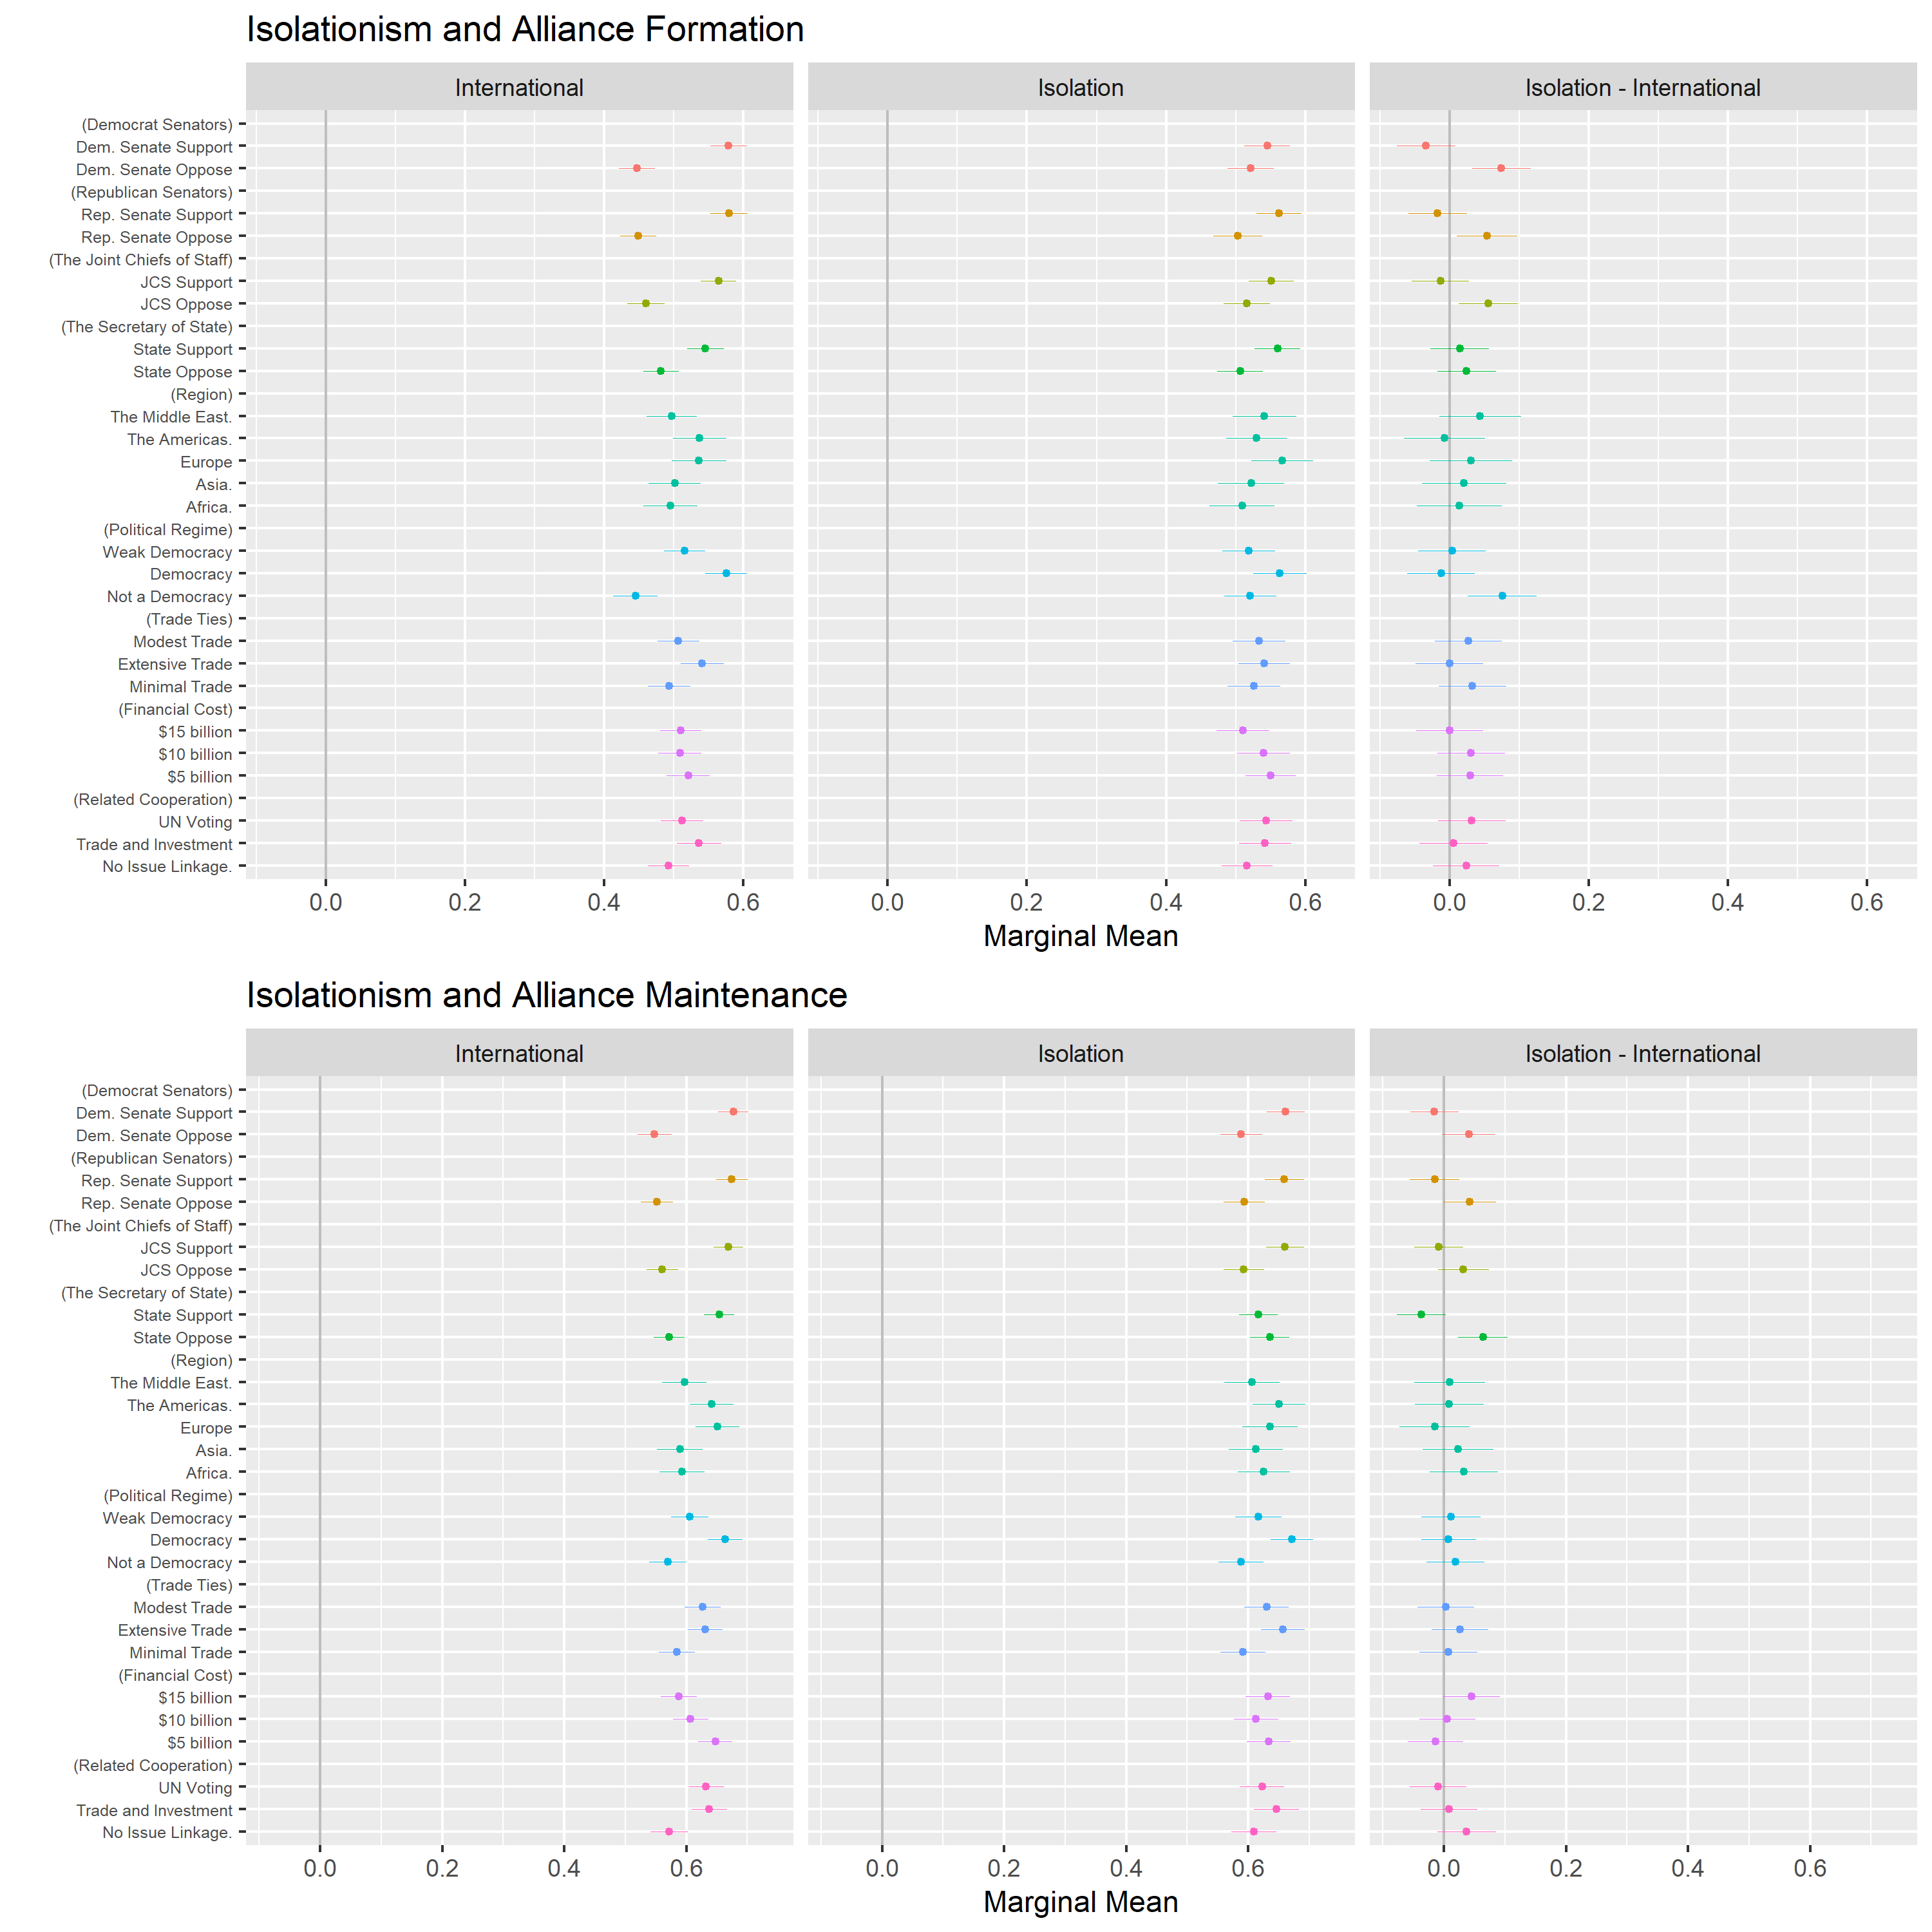
\includegraphics[width=0.95\textwidth]{isolation-plots.png}
	\caption{Marginal means of support for forming or maintaining a hypothetical alliances by partisanship. For each experiment, the left two panels plot the marginal mean of support for maintaining an alliance among isolationists and internationalists under different alliance treatments. The rightmost panel plots the difference between these groups. Components marked with abbreviated labels to make the plot more legible.}
	\label{fig:isolation-plots}
\end{figure}


\section{Treatment Interactions and Alternative Profile Distributions}


\citet{delaCuestaetal2021} observe that the distribution of profiles can affect inferences, especially when assuming a uniform distribution of profiles is problematic.
Although all the alliance profiles are feasible, some may be more likely than others. 
To investigate how this effects the AMCE estimates, I implemented the model based exploratory analysis recommendations of \citet{delaCuestaetal2021}. 


\autoref{tab:conjoint-vars-margins} summarizes the assumed marginal distributions of the different alliance attributes. 
I used data from the ATOP project \citep{Leedsetal2002} to measure the frequency of different alliance treaty obligations. 
I then make alternative assumptions about elite cues, starting with less consistent support from Republican Senators, relative to Democratic Senators, military leaders and diplomats. 
I then use the observed distribution of U.S. trade ties, the distribution of allied military capability and U.S. ally democracy to approximate the population frequency of these attributes. 
I also assume that serious common threats are unusual. 
Data on recent military cooperation is based on the size of the coalition of the willing in Iraq as a share of states in the international system. 
The assumed population distribution of financial costs is based on \citep{AlleyFuhrmann2021}. 



\begin{table}
\begin{adjustbox}{width = .99\textwidth}
\begin{tabular}{lc} 
\hline \\ 
\textbf{Attributes} & \textbf{Values} \\
\hline \\ 
Republican Senators & Support an alliance with this country. \textbf{.6} \\
                    & Oppose an alliance with this country. \textbf{.4} \\ 
                    
Democratic Senators & Support an alliance with this country. \textbf{.8} \\
                    & Oppose an alliance with this country. \textbf{.2}\\ 
                    
The Joint Chiefs of Staff & Support an alliance with this country. \textbf{.9}\\
                    & Oppose an alliance with this country.\textbf{.1}  \\ 
                    
The Secretary of State & Supports an alliance with this country. \textbf{.9} \\
                    & Opposes an alliance with this country. \textbf{.1} \\ 
% data from: https://www.census.gov/foreign-trade/Press-Release/2019pr/12/exh4s.pdf                    
Trade Ties          & The United States has minimal trade ties with this country. \textbf{.5} \\
                    & The United States has modest trade ties with this country. \textbf{.25}\\
                    & The United states has extensive trade ties with this country. \textbf{.25} \\ 
% modified from Tomz and Weeks 2013 APSR: https://web.stanford.edu/~tomz/pubs/TomzWeeks-2013-11-Appendix.pdf 
Partner Political Regime    & This country is not a democracy, and shows no sign of becoming a democracy. \textbf{.2}\\
                    & This country is a democracy, but shows signs that it may not remain a democracy. \textbf{.1} \\ % democ backsliding
                    & This country is a democracy, and shows every sign that it will remain a democracy. \textbf{.7}\\
                    
Partner Military Capability & 10,000 soldiers and spends 1\% of their GDP on the military. \textbf{.75}\\ % low
                    & 80,000 soldiers and spends 2\% of their GDP on the military. \textbf{.2} \\ % moderate
                    & 250,000 soldiers and spends 3\% of their GDP on the military. \textbf{.05}\\ % high 
                    
Shared Threat       & The United States and this country face minimal common threats. \textbf{.5} \\ 
                    & The United States and this country face modest common threats. \textbf{.35} \\
                    & The United States and this country face serious common threats. \textbf{.15} \\
% data from https://en.wikipedia.org/wiki/Multi-National_Force_%E2%80%93_Iraq                
Recent Military Cooperation  & This country has not participated in recent U.S. military operations. \textbf{.46} \\ 
                    & This country recently supported U.S. airstrikes against terrorists. \textbf{.18}\\
                    & This country recently supported U.S. counterinsurgency operations. \textbf{.18}\\
                    & This country recently fought with the United States in a war. \textbf{.18}\\
                    
Financial Cost      & This alliance requires \$5 billion in annual U.S. defense spending.  \textbf{.6}\\ 
                    & This alliance requires \$10 billion in annual U.S. defense spending.  \textbf{.3}\\ 
                    & This alliance requires \$15 billion in annual U.S. defense spending.  \textbf{.1}\\ 
                    
Conditions on Support  & The alliance treaty promises military support in any conflict. \textbf{.5} \\ 
                    & The alliance treaty promises military support only if this country is attacked. \textbf{.25} \\ 
                    & The alliance treaty promises military support only if the conflict takes place in this country's region. \textbf{.25} \\
                    
Defense Cooperation & None. \textbf{.56} \\ 
                    & The alliance treaty provides basing rights for U.S. troops. \textbf{.21}\\
                    & The alliance treaty includes a shared military command. \textbf{.07} \\
                    & The alliance treaty includes an international organization to coordinate defense policies. \textbf{.17} \\ 
% Issue linkages                    
Related Cooperation & None. \textbf{.86} \\
                    & The alliance is linked to greater trade and investment with the United States. \textbf{.07}\\ 
                    & The alliance is linked to greater support for the United States in the United Nations. \textbf{.07} \\ 
                    
Region              & Europe. \textbf{.4}\\ 
                    & Africa. \textbf{.03}\\
                    & The Middle East. \textbf{.07}\\ 
                    & Asia.\textbf{.1} \\   
                    & The Americas. \textbf{.4}\\ 
                                                                            
\hline \\
\end{tabular}
\end{adjustbox}
\caption{Table of alliance attributes in conjoint experiment profiles with alternative frequency assumptions. Frequencies for model-based population average marginal component effect estimation in bold. I use the same set of attributes as treatments in the alliance formation and maintenance experiments.} 
\label{tab:conjoint-vars-margins}
\end{table}


I use the marginal distribution of alliance attributes in \autoref{tab:conjoint-vars-margins} as the target distribution for the alliance formation experiment, but use a different procedure for the maintenance experiment. 
Rather than use an assumed distribution, I check the maintenance results using data from observed U.S. alliances as the target distribution. 
In this analysis, I use data from U.S. alliance partners in 2018 to measure the prevalence of democracy, trade ties, military capability, threat and treaty obligations. 


The population AMCE analysis has some disadvantages. 
In particular, the subgroup analyses of partisanship and foreign policy dispositions are less straightforward. 
Furthermore, I must omit the region attribute in the observed data estimates of the alliance maintenance AMCES, given the lack of U.S. alliances in Africa. 
I also have to select conditions on military support or defense cooperation values in alliances with more than one value for these attributes. 
For example, NATO has basing rights and an international organization, and I select basing rights as it is more consequential.  
Establishing the population of elite cues also required some assumptions about which alliances military and diplomatic elites would likely oppose.
While Democrat and Republican Senators have expressed skepticism of some U.S. alliances, military and diplomatic elites are usually more reticent, but some cases with opposition are necessary for this analysis. 


% quick overview of results 
\autoref{fig:pop-amce-main} and \autoref{fig:pop-amce-form} plot the population AMCE estimates, relative to the sample AMCEs reported in the manuscript. 
Even under alternative distributional assumptions, elite cues, allied democracy and financial costs exert substantial influence on alliance maintenance attitudes. 
The population AMCE estimates have much higher uncertainty, so some are not statistically significant at conventional levels, despite estimates in the same direction with greater magnitude. 



\begin{figure}
	\centering
		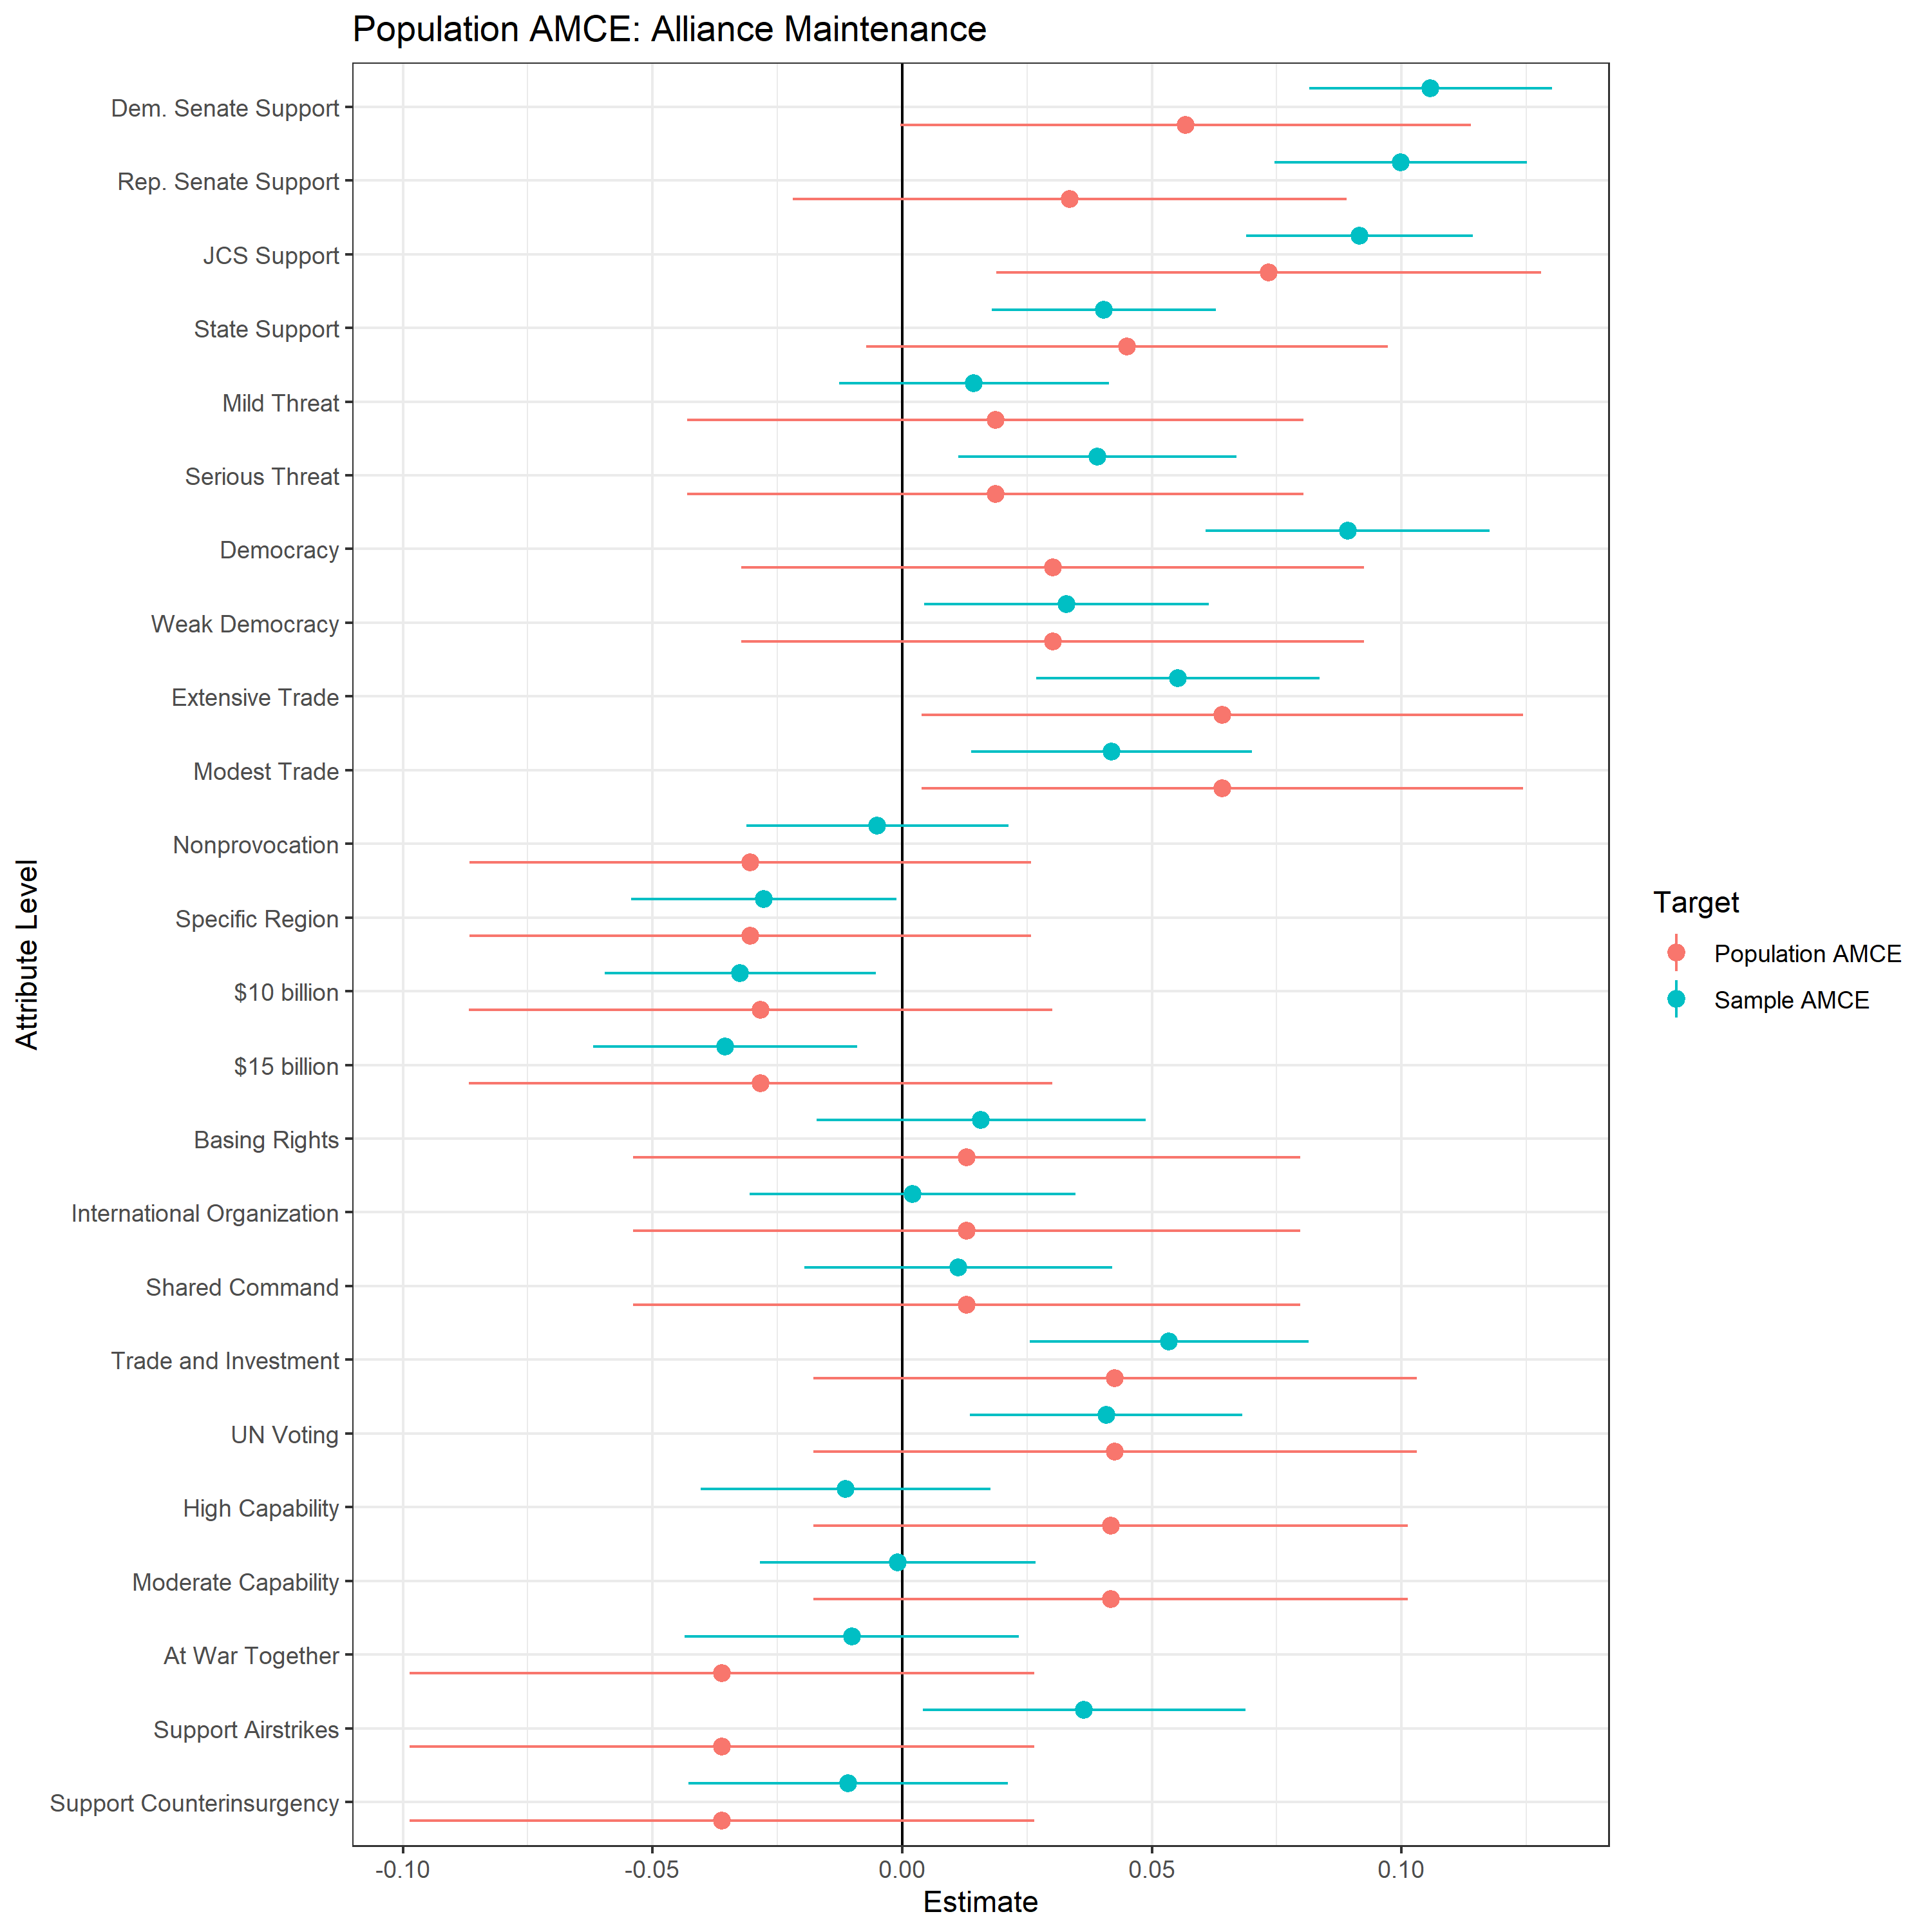
\includegraphics[width=0.95\textwidth]{pop-amce-main.png}
	\caption{Estimated AMCE of difference alliance attributes on support for alliance maintenance under alternative distributional assumptions.}
	\label{fig:pop-amce-main}
\end{figure}


\begin{figure}
	\centering
		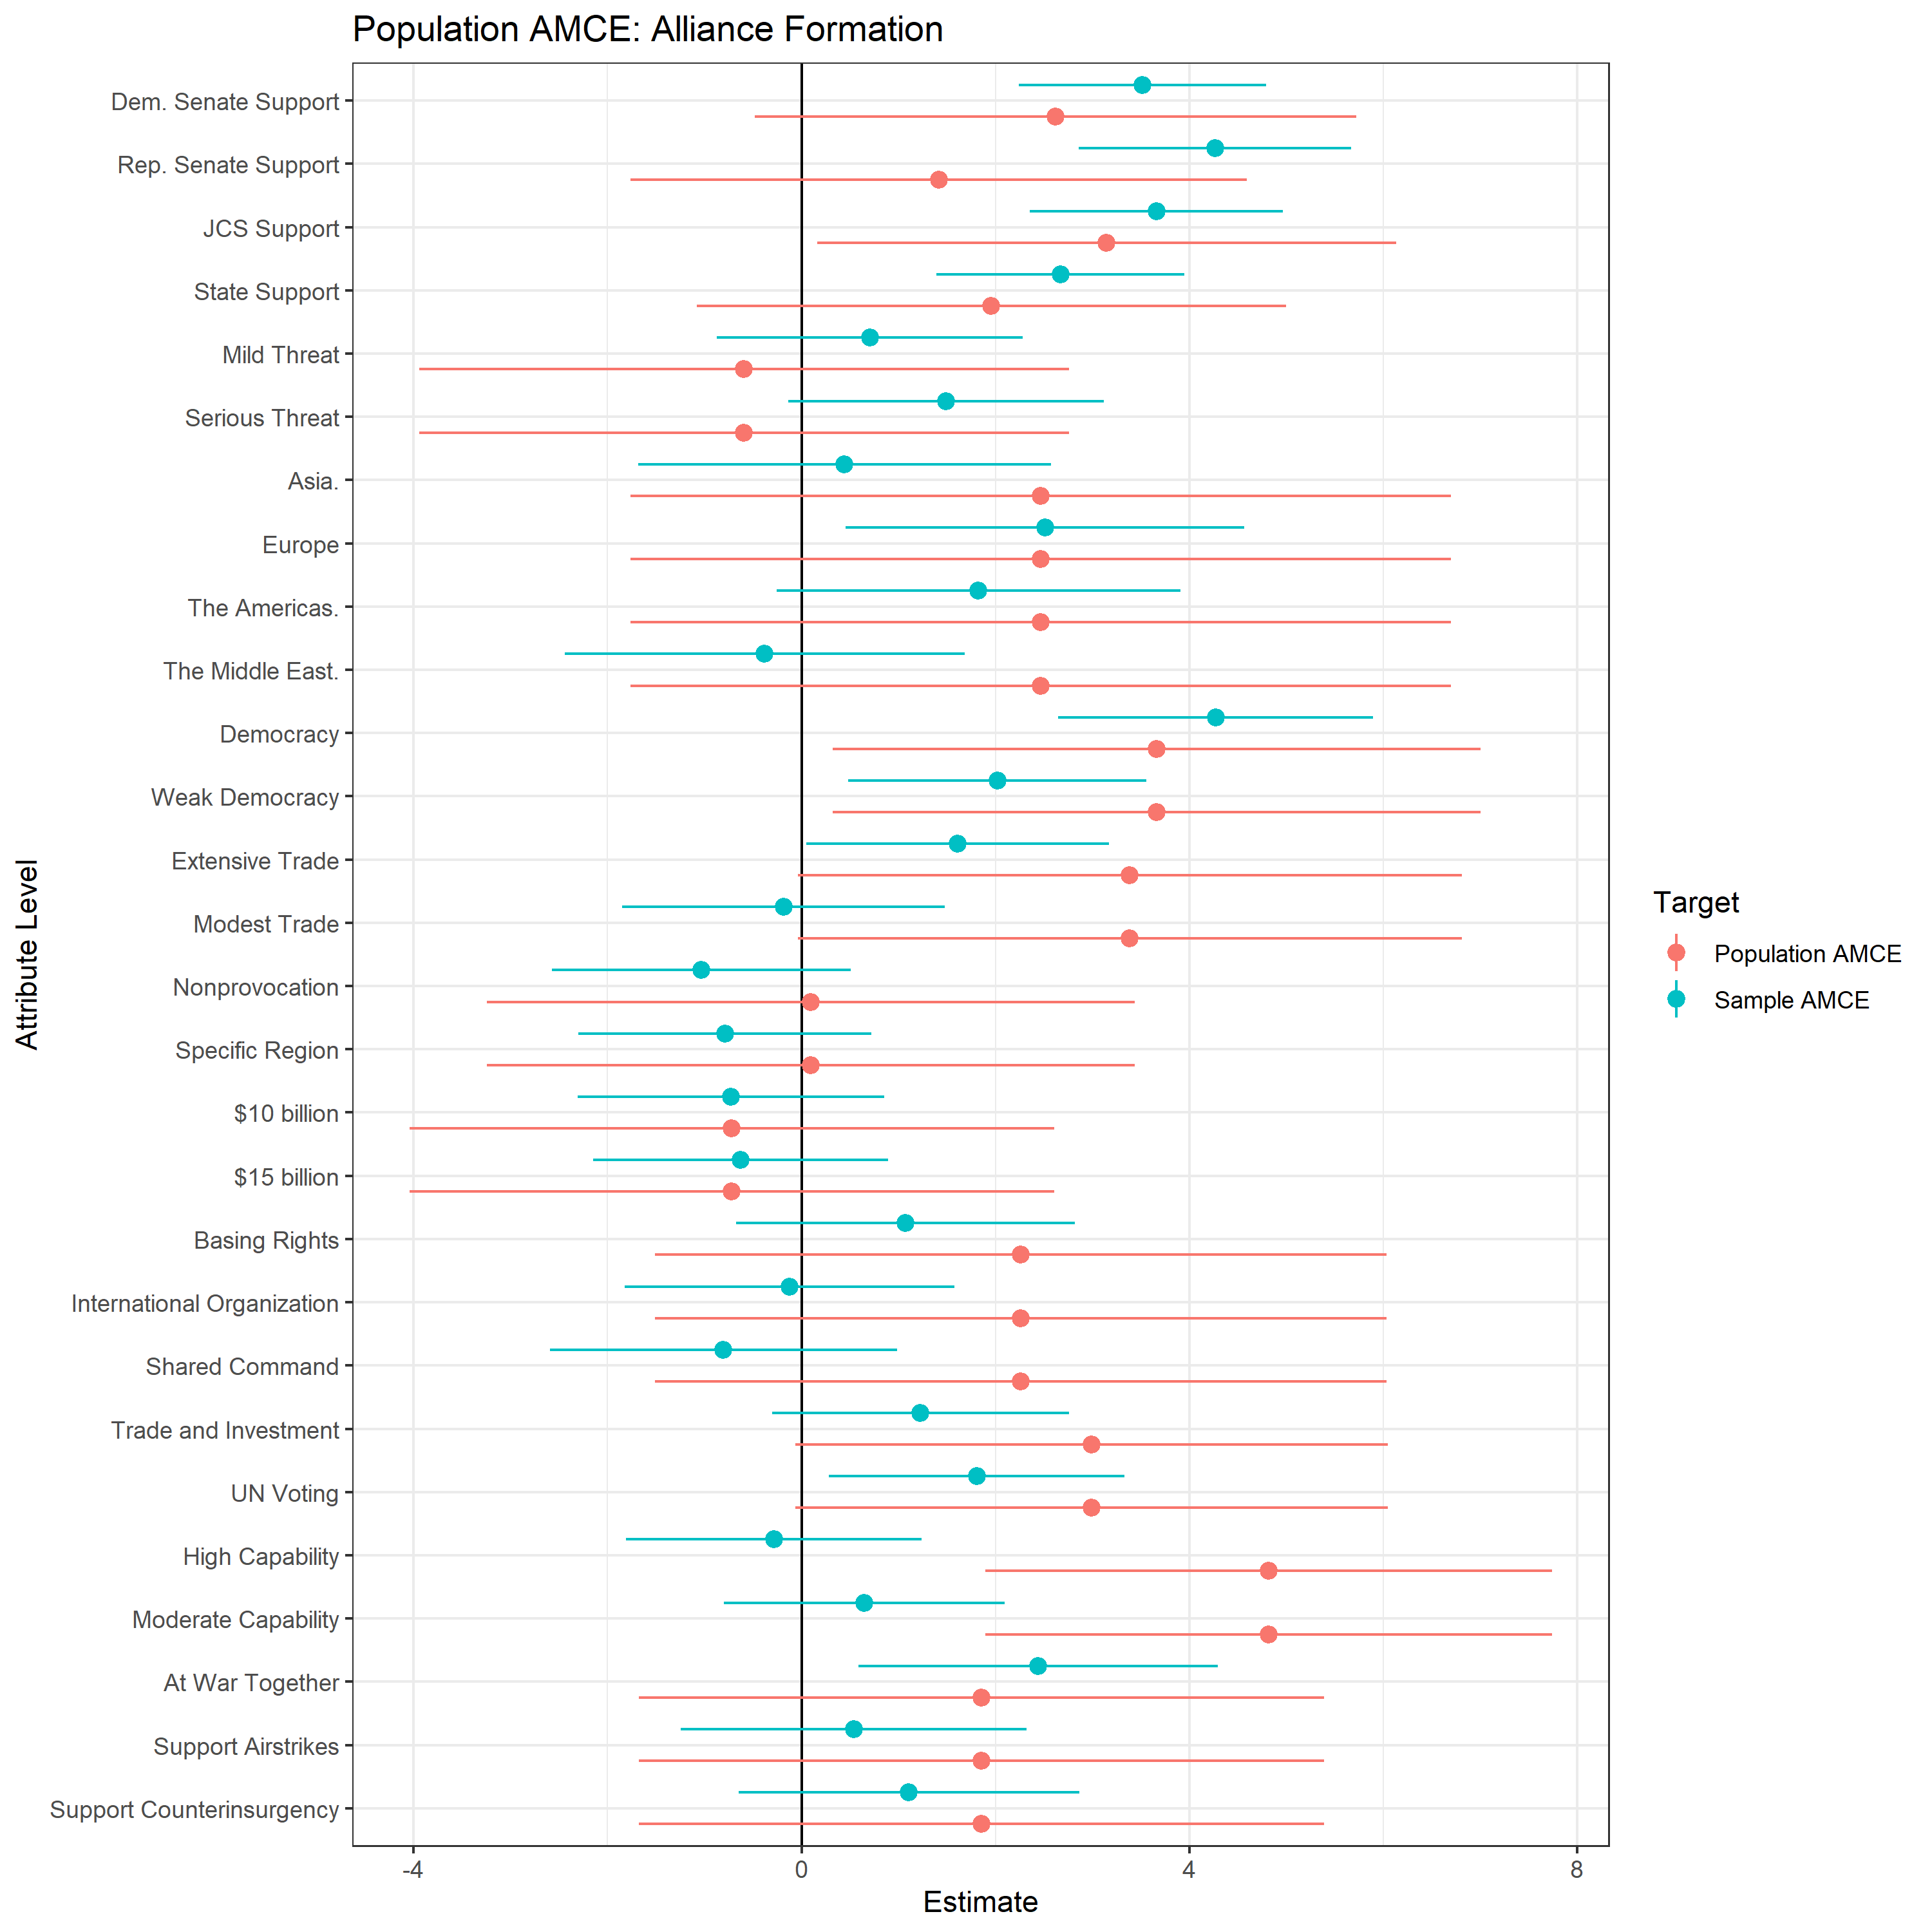
\includegraphics[width=0.95\textwidth]{pop-amce-form.png}
	\caption{Estimated AMCE of difference alliance attributes on support for alliance maintenance under alternative distributional assumptions.}
	\label{fig:pop-amce-form}
\end{figure}

% summarize differences
There are also some differences between the population and sample AMCE estimates. 
Trade exerts a stronger influence on alliance attitudes under different marginal distributions of the attributes. 
In the alliance formation experiment, elite cues are less influential than allied democracy, trade and capability. 


\section{Open-Ended Alliance Attitudes} 


To further examine the primary sources of alliance attitudes, I asked respondents to identify the most important factors behind their support or opposition to the hypothetical alliances in an open-ended question. 
Roughly half of the respondents gave no response or useless answers, which limits the utility of the responses below. 
It does provide some useful insight into the personal characteristics that predict particular emphases in alliance attitudes, however. 


Based on a reading of the open-ended questions, I created three dummy indicators of general alliance attributes. 
The first takes on a value of one for mentions of elite cues using the generic elite, bipartisan, partisan, military, and diplomatic cues indicators. 
The second has a value of one if a respondent references alliance partner attributes through the trade, regime type, threat, region, recent military cooperation and capability dummies. 
The last indicator captures any mention of alliance obligations, including cost, issue linkages, defense cooperation and conditions on military support. 
These three variables are not mutually exclusive, because respondents often mentioned multiple factors from different categories. 


Because individuals highlight multiple alliance attributes, I analyze the open-ended responses with a Bayesian multivariate probit model, which captures correlations between the different response classes. 
Each equation of the model predicts open-ended response content using individual characteristics, including the strength of individual partisan attachment, international economic interests, gender, race, education, region and income. 
Because the model has many parameters, I employ Bayesian estimation to regularize the estimates. 


\newpage

% Bibliography
 
\bibliography{../../MasterBibliography} 


\end{document}
